 \documentclass[12pt,a4paper]{article}

\usepackage{graphicx}% Include figure files
\usepackage{dcolumn}% Align table columns on decimal point
\usepackage{bm}% bold math
%\usepackage{hyperref}% add hypertext capabilities
%\usepackage[mathlines]{lineno}% Enable numbering of text and display math
%\linenumbers\relax % Commence numbering lines

%\usepackage[showframe,%Uncomment any one of the following lines to test 
%%scale=0.7, marginratio={1:1, 2:3}, ignoreall,% default settings
%%text={7in,10in},centering,
%%margin=1.5in,
%%total={6.5in,8.75in}, top=1.2in, left=0.9in, includefoot,
%%height=10in,a5paper,hmargin={3cm,0.8in},
%]{geometry}

\usepackage{multicol}%Para hacer varias columnas
\usepackage{multicol,caption}
\usepackage{multirow}
\usepackage{cancel}
\usepackage{hyperref}
\hypersetup{
    colorlinks=true,
    linkcolor=blue,
    filecolor=magenta,      
    urlcolor=cyan,
}

\setlength{\topmargin}{-1.0in}
\setlength{\oddsidemargin}{-0.3pc}
\setlength{\evensidemargin}{-0.3pc}
\setlength{\textwidth}{6.75in}
\setlength{\textheight}{9.5in}
\setlength{\parskip}{0.5pc}

\usepackage[utf8]{inputenc}
\usepackage{expl3,xparse,xcoffins,titling,kantlipsum}
\usepackage{graphicx}
\usepackage{xcolor} 
\usepackage{siunitx}
\usepackage{nopageno}
\usepackage{lettrine}
\usepackage{caption}
\renewcommand{\figurename}{Figura}
\usepackage{float}
\renewcommand\refname{Bibliograf\'ia}
\usepackage{amssymb}
\usepackage{amsmath}
\usepackage[rightcaption]{sidecap}
\usepackage[spanish]{babel}

\providecommand{\abs}[1]{\lvert#1\rvert}
\providecommand{\norm}[1]{\lVert#1\rVert}
\newcommand{\dbar}{\mathchar'26\mkern-12mu d}

\usepackage{mathtools}
\DeclarePairedDelimiter\bra{\langle}{\rvert}
\DeclarePairedDelimiter\ket{\lvert}{\rangle}
\DeclarePairedDelimiterX\braket[2]{\langle}{\rangle}{#1 \delimsize\vert #2}

% CABECERA Y PIE DE PÁGINA %%%%%
\usepackage{fancyhdr}
\pagestyle{fancy}
\fancyhf{}

\begin{document}

Macías Márquez Misael Iván

\begin{enumerate}



%%%1%%%



\item Dos personas están en reposo y separadas por una distancia $L$ a lo largo de una carretera. Las personas aplauden simultáneamente en el sistema de referencia de la carretera. En el marco de referencia de un auto que va de izquierda a derecha sobre la carretera con velocidad $v$ ¿Qué persona aplaudió primero? ¿A qué tiempo?

\textbf{Sol:}

Pongamos nuestro sistema de referencia en la persona de la izquierda, entonces sea la posición de la persona de la izquierda $x_1= 0$ y de la otra $x_2=L$,como el aplauso sucedió al mismo tiempo en el sistema de referencia en reposo los tiempos del suceso para cada persona son $t_1 = t_2 = t_0 > 0$, ahora para el sistema de referencia del auto con velocidad $v$ usando las transformaciones de Lorentz las posiciones y tiempos de cada persona son:

\begin{equation*}
    x'_1 = \gamma (x_1 - v t_1)= \gamma (0 - v t_0) = \gamma v t_0 \hspace{2cm} t'_1 = \gamma (t_1 - \frac{vx_1}{c^2}) =  \gamma (t_0 - \frac{v0}{c^2}) = \gamma t_0
\end{equation*}

\begin{equation*}
    x'_2 = \gamma (x_2 - v t_2)= \gamma(L - vt_0) \hspace{2cm} t'_1 = \gamma (t_1 - \frac{vx_1}{c^2})=\gamma (t_0 - \frac{vL}{c^2})
\end{equation*}

entonces como $vL/c^2 > 0$, $t'_1 > t'_2$ por lo que la segunda persona aplaudió primero en el marco de referencia en movimiento. Nótese que si $v << c$ entonces $v/c << 1$ y los tiempos $t'_1$ y $t'_2$ resultan ser iguales.





%%%2%%%



\item El eje temporal de un observador $S'$, son los puntos que satisfacen $x'=0$ y su línea de mundo se ve en el diagrama de espacio tiempo de $S$ como una recta que hace un ángulo $\alpha$ con el eje $t$, además, está relacionado con la velocidad relativa $v$ como:$\tan{\alpha} = 1/v$. Muestre que el ángulo que hace el eje $x'$ con el eje $x$ es también $\alpha$.

\textbf{Sol:}

Un observador que se mueve a una velocidad constante describe una recta donde la pendiente/velocidad es:

\begin{equation*}
    v = \frac{x}{t}
\end{equation*}


\begin{figure}[h!]
    \centering
    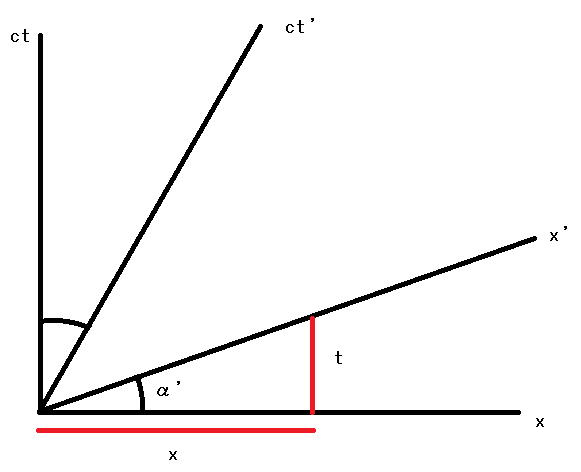
\includegraphics[scale=0.5]{rela1.png}
    \caption{}
    \label{fig:my_label}
\end{figure}

en la figura 1 también se puede ver que esta recta forma un triangulo rectángulo con un ángulo $\alpha'$ donde además se cumple que

\begin{equation*}
    \tan{\alpha'}= \frac{t}{x} = \frac{1}{\frac{x}{t}} = \frac{1}{v}
\end{equation*}

\newpage
por lo tanto el angulo formado por el eje $x'$ y $x$ es el mismo que el formado por el eje $t$ y $t'$ ($\alpha= \alpha'$).





%%%3%%%



\item Una varilla se mueve de derecha a izquierda con una velocidad $v_1 = 3c/5$ con respecto al piso. La longitud de la varilla en el sistema del piso es $L$. Para un observador se mueve hacia la derecha con una velocidad $v_2=c/2$ con respecto al piso. ¿Cuál es la longitud de la varilla?

\textbf{Sol:}

Como se vio en clase, pero ahora con velocidades en sentidos contrarios y suponiendo que se estén alejando, se tiene que

\begin{equation*}
    x' = \gamma (x + v_2 t) \hspace{1cm} t' = \gamma (t + \frac{v_2x}{c^2})
\end{equation*}

o bien

\begin{equation*}
    dx' = \gamma (dx + v_2 dt) \hspace{1cm} dt' = \gamma (dt + \frac{v_2dx}{c^2})
\end{equation*}

por lo que la velocidad en el sistema primado es

\begin{equation}
    u' = \frac{dx'}{dt'} =\frac{\cancel{\gamma}(dx+vdt)}{\cancel{\gamma}(dt+\frac{v}{c^2}dx)} = \cancel{\frac{dt}{dt}} \frac{\frac{dx}{dt} + v_2}{1 + \frac{v_1 }{c^2} \frac{dx}{dt}}= \frac{v_1+v_2}{1+\frac{v_1 v_2}{c^2}} = 0.85 c
\end{equation}

por lo tanto la longitud de la varilla para el observador a $t=0$ es de

\begin{equation*}
    x' = \gamma (L+\cancel{u't})=  1.89 L 
\end{equation*}



%%%4%%%



\item Dos eventos ocurren en el mismo lugar en el sistema de referencia del laboratorio y están separados en tiempo por 3 segundos.

\begin{itemize}
    \item ¿Cuál es la distancia espacial entre éstos dos eventos en un sistema de referencia de una nave en la que los eventos separados 6 segundos?
    
    \textbf{Sol:}
    
    Sea $x_1$ y $x_2$ la posición de los 2 evento, también sea $t_1$ y $t_2$ los tiempos de cada evento en el sistema de referencia del laboratorio que por hipótesis $t_2 = t_1 +3s$ y $v_{rel}$ la velocidad de la nave entonces por la transformada de Lorentz, la diferencia de longitudes en el sistema de la nave es:
    
    \begin{equation*}
        \Delta x' = \gamma (x_1 - x_2 + \cancel{v_{rel}t_1 - v_{rel}t_2}) = \gamma (x_1 - x_2)
    \end{equation*}
    
    pero los eventos ocurrieron en el mismo lugar en el sistema de referencia del laboratorio por lo que $x_1 = x_2$ y entonces $\Delta x' = 0$
    
    
    \item ¿Cuál es la velocidad relativa $v_{rel}$ entre la nave y el laboratorio?
    
    \textbf{Sol:}
    
    \begin{equation*}
        \Delta t' = \gamma (t_1 - t_2 + \cancel{\frac{v_{rel}x_1}{c^2} - \frac{v_{rel} x_2 }{c^2}}) = \gamma (t_1 - t_1 + 3s) = 3\gamma s= 6s
    \end{equation*}
    
    por lo que $\gamma = 2$
    
    \begin{equation*}
        \gamma = \frac{1}{\sqrt{1 - \frac{v_{rel}^{2}}{c^2}}} = 2 \hspace{0.3cm} \rightarrow \hspace{0.3cm} v = \frac{\sqrt{3}}{2} c
    \end{equation*}
    
    
    
\end{itemize}




%%%5%%%



\item El tren $A$ con longitud propia $L$ se mueve de izquierda a derecha con velocidad $v$ con respecto al sistema de la vía. El tren $B$ se mueve paralelamente pero en dirección contraria (de derecha e izquierda) también con velocidad $v$ con respecto a la vía.¿Cuánto tiempo pasa entre que los frentes de los trenes coinciden y parte de atrás coinciden?

\begin{itemize}
    \item En el sistema de $A$
    
    \textbf{Sol:}
    
    Usando la ecuación 1 del ejercicio 3, la velocidad del tren $B$ desde el sistema de $A$ es:
    
    \begin{equation*}
        v' = \frac{v+v}{1 + \frac{vv}{c^2}} = \frac{2v}{1 + \frac{v^2}{c^2}}
    \end{equation*}
    
    entonces como
    
    \begin{equation*}
        v' = \frac{\Delta x'}{\Delta t'} \hspace{0.3cm} \rightarrow \hspace{0.3cm} \Delta t' = \frac{\Delta x'}{v'}= \frac{\gamma (\Delta x + v' (\Delta t))}{v'} = \gamma \frac{L + v' \Delta t}{v'}
     \end{equation*}
    
    \item En el sistema de la vía
    
    \textbf{Sol:}
    
    Poniendo el origen del sistema  justo en el punto donde los trenes se encuentran, se tiene que
    
    \begin{equation*}
        \Delta x' = v\Delta t'_1 + v \Delta t'_2 
    \end{equation*}
    
    que al ser de la misma longitud e ir a la misma velocidad se puede reducir como
    
    \begin{equation*}
        \Delta x' = 2v\Delta t'\hspace{0.3cm} \rightarrow \hspace{0.3cm} \Delta t' = \frac{\Delta x'}{2v} = \frac{\gamma(\Delta x + v \Delta t)}{2v} = \gamma \frac{2 \Delta x}{2v} = \gamma \frac{L}{v}
    \end{equation*}
    
\end{itemize}



%%%6%%%



\item Convierta las siguientes cantidades a sus equivalentes en unidades geométricas con $c=1$:

\begin{itemize}
    \item La constante de Planck $\hbar = 1.05 \times 10^{-34} J \cdot s$
    
    \textbf{Sol:}
    
    \begin{equation*}
        [J] = \frac{kg m^2}{s^2} \hspace{1cm} \rightarrow \hspace{1cm} Js = \frac{kg m^2}{s}
    \end{equation*}
    
    entonces al ser $c=1$ se tiene que $1s = 3 \times 10^8 m$ por lo que pasando los metros a segundos en la constante de Planck se tiene
    
    \begin{equation*}
        h = 1.05 \times 10^{-34} \frac{1}{(3\times 10^8)^2} kg s= 1.17 \times 10^{-51} kg s
    \end{equation*}
    
    y ahora pasando segundo a metros
    
    \begin{equation*}
        h = 1.05 \times 10^{-34} \frac{1}{3\times 10^8} kg m= 3.5 \times 10^{-43} kg m
    \end{equation*}
    
    
    \item Momento de una partícula $p = 3 \times 10^4 kg m s^{-1}$
    
    \textbf{Sol:}
    
    de metros a segundos
    
    \begin{equation*}
        p = \frac{3 \times 10^4}{3\times 10^8} kg = 1\times 10^{-4} kg
    \end{equation*}
    
    y de segundos a metros
    
    \begin{equation*}
        p = \frac{3 \times 10^4}{3\times 10^8} kg = 1\times 10^{-4} kg
    \end{equation*}
    
    
    \item Presión atmosférica $P=1 \times 10^{5} N m^{-2}$
    
    \textbf{Sol:}
    
    \begin{equation*}
        [N] = kg \frac{m}{s^2} \hspace{1cm} \rightarrow \hspace{1cm} N/m^2 = \frac{kg}{s^2 m}
     \end{equation*}
     
     entonces de metros a segundos
     
     \begin{equation*}
         P = (1 \times 10^5) (3 \times 10^{8}) \frac{kg}{s^3} = 3 \times 10 ^{13} \frac{kg}{s^3}
     \end{equation*}
     
     
     y de segundos a metros
     
     \begin{equation*}
         P = \frac{1\times 10^{5}}{(3 \times 10 ^8)^2} \frac{kg}{m^3} = 1.11 \times 10^{-12  }\frac{kg}{m^3}
     \end{equation*}
    
\end{itemize}



    
    
\end{enumerate}

\end{document}

